\documentclass{article}
\usepackage[utf8]{inputenc}
\usepackage[spanish]{babel}
\usepackage{graphicx}
\usepackage{float}
\usepackage{hyperref}

\title{Práctica 3. Desarrollo de una aplicación multiplataforma}
\author{Noelia Escalera Mejías \and Jesús Torres Sánchez}

\begin{document}
	\maketitle
	\tableofcontents
	\newpage
	
	\section{Descripción}
	Se ha decidido implementar una aplicación de votaciones conjuntas siguiendo un modelo cliente-servidor. Por un lado tendremos un servidor que se encarga de recoger los distintos datos de las votaciones y tendremos una página que muestra dichos resultados. Por otro tendremos otra página mediante la cuál los usuarios podrán crear o unirse a salas de votación y/o votar en distintas votaciones.
	
	\section{Requisitos funcionales}
	\begin{itemize}
		\item \textbf{RF-1.} Alta de usuario.
		\item \textbf{RF-2.} Unirse a votación.
		\item \textbf{RF-3.} Crear una sala de votación.
		\item \textbf{RF-4.} Votar en una votación.
		\item \textbf{RF-5.} Consultar resultados.
		\item \textbf{RF-6.} Seleccionar tipo de votación. \\
	\end{itemize}
	
	\section{Requisitos no funcionales}
	\begin{itemize}
		\item \textbf{RNF-1}. La interfaz gráfica será sencilla con el objetivo de facilitar el uso para la mayoría de usuarios.
		\item \textbf{RNF-2.} Al establecer comunicaciones con un servidor web debemos tener
		en cuenta múltiples aspectos de seguridad tanto en la propia aplicación
		como en el servidor en sí.
		\item \textbf{RNF-3}. La aplicación tiene que tener facilidad para ser portable.
		\item \textbf{RNF-4}. El servidor debe estar disponible en todo momento para poder
		acceder a las distintas votaciones en tiempo real.
		\item \textbf{RNF-5}. Habrá una amplia variedad de votaciones para elegir.
	\end{itemize}

	\section{Listado de las partes interesadas y de las preocupaciones de cada una}
	\begin{itemize}
		\item {\bf Arquitecto.} Sus principales preocupaciones son que el sistema pueda ser portable y multiplataforma.
		\item {\bf Cliente (Adquiriente).} Que la aplicación sea atractiva para distintos usuarios.
		\item {\bf Desarrollador.} Conseguir un código legible y fácilmente actualizable.
		\item {\bf Servicio al cliente.} Contar con una manera fácil de comunicarse con el cliente.
		\item {\bf Administrador del sistema.} 
		\item {\bf Técnico de pruebas.} 
		\item {\bf Usuarios.} Que la interfaz sea intuitiva y que el servidor esté disponible el mayor tiempo posible.
	\end{itemize}

	\section{Listado de criterios de calidad}
	\begin{itemize}
		\item {\bf Gestión del producto.} Consideramos el sistema como un producto para evaluar la evolución en su conjunto.
		\item {\bf Magnitud de cambio.} Si apreciamos esto, se evitarán grandes costos.
		\item {\bf Dimensión del cambio.} A nivel funcional, de plataforma, de integración y de crecimiento de uso.
		\item {\bf Probabilidad del cambio.} Hay que ser muy precisos en la apreciación de que los cambios sean realmente necesarios.
		\item {\bf Temporización del cambio.} Hay que estimar el momento probable para realizar cambios.
		\item Elegir el momento del cambio equilibrando los costes de desarrollo (mayores a mayor flexibilidad del sistema a desarrollar) y los costes de mantenimiento (mayores a mayor velociad en el desarrollo).
		\item Considerar los cambios impuestos por factores externos (fin de la vida útil, cambios en la población de usuarios o perfiles, etc).
		\item Preservar el conocimiento mediante alguna documentación para cuando cambie el equipo de mantenimiento.
		\item Probar los cambios (automatizar las pruebas, hacer una buena gestión de la configuración, abstraer procesos repetibles).
	\end{itemize}


	\section{Diagrama de componentes}
	A partir de los requisitos mencionados anteriormente, podemos obtener el siguiente diagrama de cajas y líneas, que muestra las características del sistema a nivel contextual:
	
	\begin{figure}[H]
		\centering
		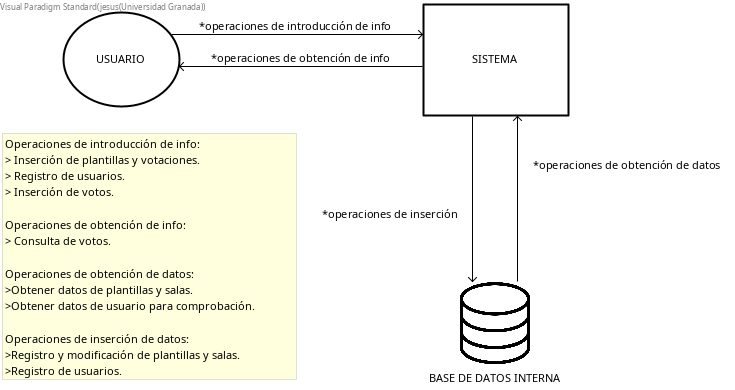
\includegraphics[totalheight=7.5cm]{img/diagrama_cajas}
		\caption{Diagrama contextual}
	\end{figure}

	\section{Diagrama de clases de diseño}
	A continuación se adjunta un diagrama de clases de diseño, dónde se especifican los elementos más importantes del sistema así como las relaciones entre los mismos:
	
	\begin{figure}[H]
		\centering
		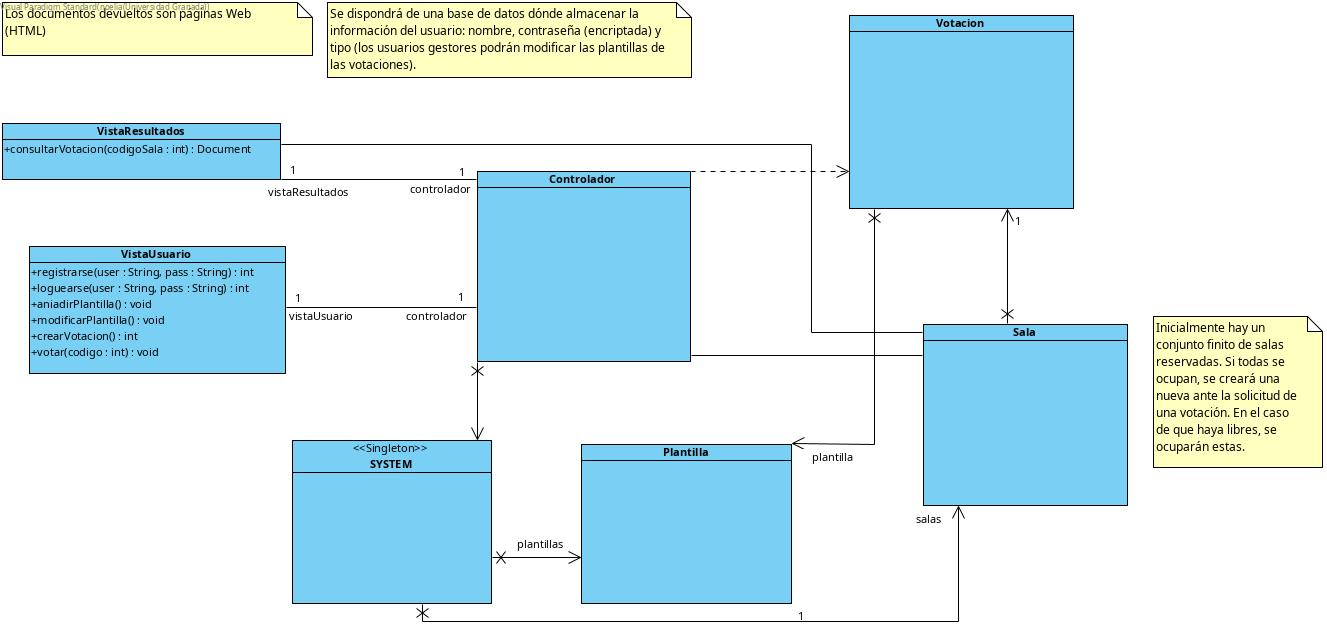
\includegraphics[totalheight=7cm]{img/5.jpg}
		\caption{Diagrama de clases de diseño}
	\end{figure}
	
	\section{Problemas encontrados con tecnologías finalmente no aplicadas}
	\subsection{Angular JS y Firebase}
	Nuestra primera idea fue desarrollar la aplicación para móvil. En primer lugar, intentamos utilizar Angular JS y Firebase, para ello, intentamos seguir el siguiente 
	 \href{https://medium.com/@rotemtam/build-a-kahoot-clone-with-angularjs-and-firebase-b8b30891d968}{tutorial}. No nos quedó claro cómo conectar Firebase a la aplicación, ya que no daba muchos detalles. Además, el enlace de la demo de la página está roto. Al llegar al paso de usar el generador angular-fire, te pide una instancia de Firebase, no dejaba muy claro qué había que poner.
	 
	 \begin{figure}[H]
	 	\centering
	 	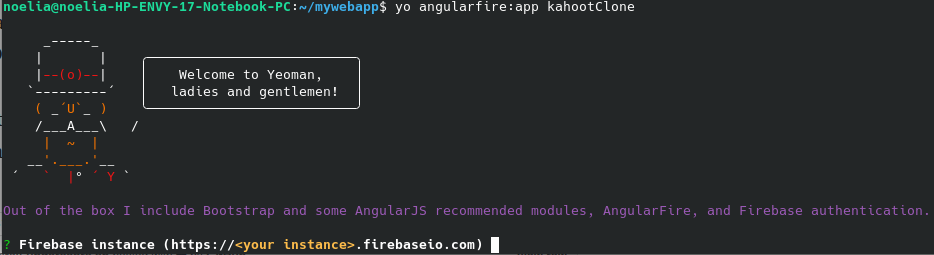
\includegraphics[totalheight=3.35cm]{img/1.png}
	 \end{figure}
 
 	Una vez conseguimos averiguar qué nos pedía, ejecutamos la orden y nos dio el siguiente error:
 	
 	\begin{figure}[H]
 		\centering
 		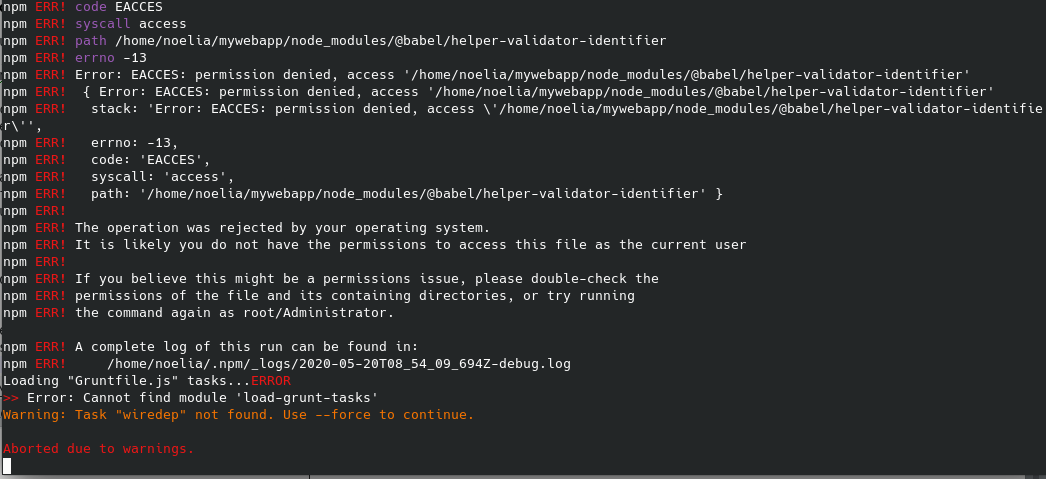
\includegraphics[totalheight=5.5cm]{img/2.png}
 	\end{figure}
 	\subsection{Firebase y App Engine}
 	Nos pareció interesante la tecnología Firebase e
 	e investigamos sobre cómo conectarnos desde una aplicación. Encontramos el siguiente \href{https://cloud.google.com/solutions/mobile/mobile-firebase-app-engine-flexible}{tutorial}. Tras varias horas de trabajo, conseguimos llegar hasta casi el final del tutorial, hasta que llegó un momento en que para seguir se nos pedía la tarjeta de crédito por parte de Firebase. Se supone que no te hacían ningún tipo de cargo, pero no nos gustó la idea. Además nos apareció el siguiente error al intentar ejecutar el servicio en el servidor local con {\bf \$mvn clean package appengine:run}
 	\begin{figure}[H]
 		\centering
 		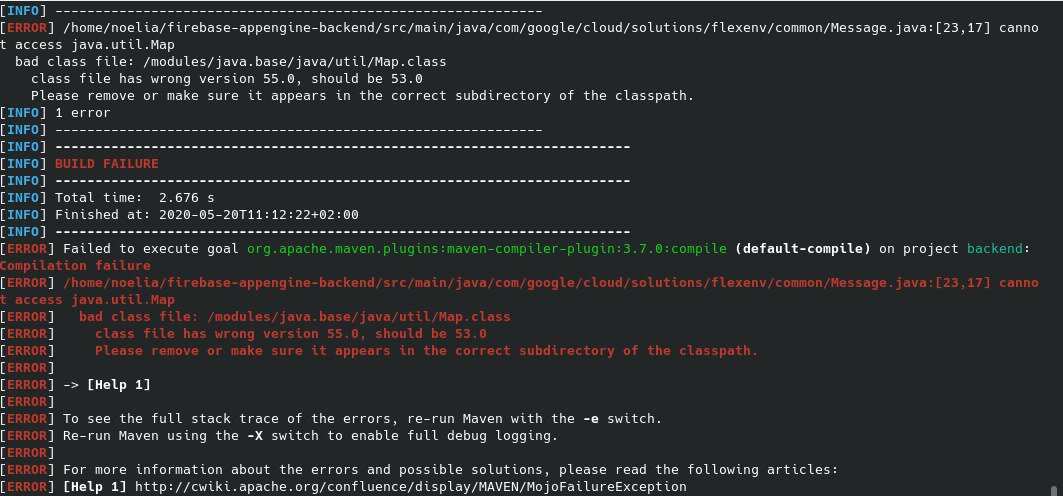
\includegraphics[totalheight=5.7cm]{img/3.png}
 	\end{figure}
 	\subsection{Android JS}
 	También intentamos usar Android JS, para ello seguimos este \href{https://blog.usejournal.com/how-to-build-android-apps-with-node-js-using-android-js-2aa4643be87b}{tutorial}. Tras seguirlo hasta el final, daba este error al empaquetar:
 	\begin{figure}[H]
 		\centering
 		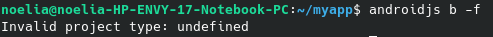
\includegraphics[totalheight=0.92cm]{img/4.png}
 	\end{figure}
 	\section{Tecnologías finalmente usadas}
 	Finalmente decidimos hacer la aplicación para web, hemos usado las siguientes tecnologías:
 	\subsection{Node JS}
 	Es un entorno de ejecución multiplataforma, de código abierto para la capa del servidor, basado en JavaScript, asíncrono, con E/S de datos en una arquitectura orientada a eventos y vasado en el motor V8 de Google. Para utilizarlo nos hemos servido de lo aprendido en la asignatura Desarrollo de Sistemas Distribuidos, así como en distinta documentación de internet.
 	\subsection{Express JS}
 	Es una infraestructura de aplicaciones web Node.js mínima y flexible que proporciona un conjunto solido de características para las aplicaciones web y móviles. Nos ha servido de gran utilidad para manejar las sesiones de los usuarios, así como para manejar las redirecciones, entre otras cosas. Nos han sido de gran utilidad los tutoriales que proporciona su página web: \url{https://expressjs.com/es/}.
 	\subsection{MongoDB}
 	Se trata de un sistema de base de datos NoSQL, orientado a documentos y de código abierto, que es muy fácil de usar junto con Node. Lo hemos usado para guardar las cuentas de los usuarios, las encuestas, etc. Para usarlo nos hemos servido de lo aprendido en Desarrollo de Sistemas Distribuidos, así como de bibliografía de internet cuando nos surgían dudas.
 	\subsection{EJS}
 	EJS o Embebed Javascript Templating, es un motor de plantillas, que permite generar HTML con JavaScript. Nos ha sido muy útil la ayuda de la página oficial: \url{https://ejs.co/}.
 	\subsection{HTML}
 	Por supuesto, hemos tenido que usar HTML como base para las distintas páginas de la aplicación.
 	
 	\section{Funcionamiento de la aplicación}
 	Partiendo de los requisitos y criterios de calidad mencionados anteriormente, se ha decidido crear una página web usando las tecnologías previamente comentadas. \\
 	Al acceder a la página web, lo primero que nos encontramos es la opción de log-in, ya que es un requisito imprescindible estar identificado previamente para poder acceder al sistema. Adicionalmente, en el caso de que no estemos registrados, nos proporcionará una alternativa para poder registrarnos. \\
 	Este proceso se llevará a cabo gestionando las distintas peticiones en el servidor por medio de Express, y comprobando las credenciales a partir de la información almacenada en la base de datos. \\ ~\\
 	
 	Una vez nos hemos identificado o registrado, podremos acceder al menú principal. Este menú nos proporciona una serie de operaciones:
 	\begin{itemize}
 		\item Una operación de acceso a la sala. Para poder realizar esta operación debemos proporcionar un código de sala válido. Una sala es válida si tiene asociada una votación con una fecha de finalización posterior a la fecha actual y una fecha de inicio anterior a la actual. Es decir, la votación de la sala actual debe estar en curso para que podamos acceder a la misma.
 		
 		\item Una operación de votación en una sala. Para poder votar en la sala, además de cumplir los requisitos de acceso mencionados anteriormente, también debemos comprobar que el usuario presenta permisos para participar en esta votación.
 		
 		\item Una operación para añadir un usuario a la lista de miembros de una votación. El usuario podrá realizar esta operación sobre todas las votaciones creadas por el mismo.
 		
 		\item Una operación para añadir una plantilla, especificando: el nombre de la plantilla, las distintas preguntas y las alternativas para cada pregunta.
 		
 		\item Una operación para añadir una votación, especificando: el nombre de la votación, la plantilla a usar, la fecha de inicio de la votación y la fecha de finalización. En el caso de que las fechas proporcionadas no sean válidas, generará los avisos correspondientes.
 		
 		\item Adicionalmente, se permitirá que el usuario se desloguee, destruyendo la sesión correspondiente.
 	\end{itemize}
 
 	Para poder desarrollar este proceso correctamente, requerimos disponer de información almacenada, sobre todo en cuanto a los usuarios, las votaciones asociadas a las salas y las plantillas disponibles. Para ello, haremos uso de una base de datos MongoDB, cargando cada vez que arranca el sistema la información correspondente y actualizándola cada vez que se modifique. Por ejemplo, en el caso de las votaciones asociadas a las salas, cada vez que se cree una nueva votación, se comprobarán todas las salas asignadas de forma secuencial: si una sala tiene asociada una votación que ya ha expirado, podemos asignarle dicha sala a la votación en cuestión. \\
 
 	En las siguientes capturas de pantalla se muestra el ejemplo de una votación sencilla, permitiéndonos observar de forma práctica el funcionamiento del sistema:
 	\newpage
 	
 	En primer lugar nos registramos:
 	\begin{figure}[H]
 		\centering
 		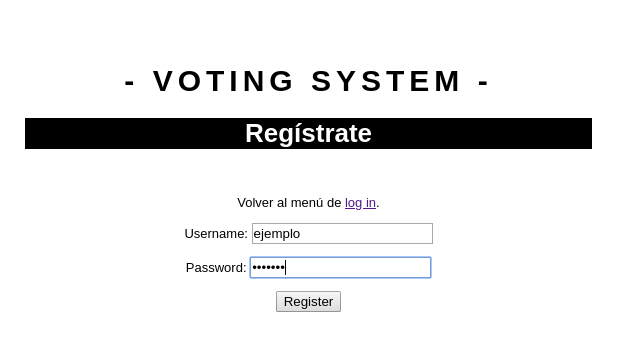
\includegraphics[totalheight=6.5cm]{img/cap6}
 		\caption{}
 	\end{figure}
 ~\\
 
 	O en el caso de que estuviésemos previamente registrados, iniciamos sesión:
 	\begin{figure}[H]
 		\centering
 		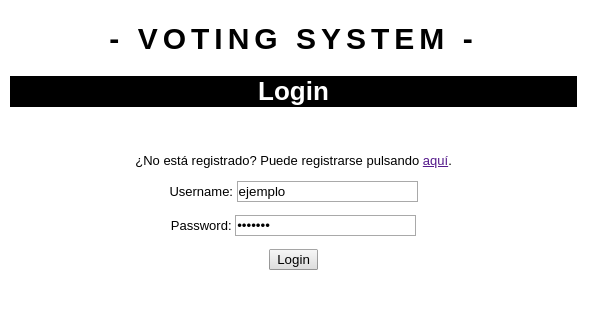
\includegraphics[totalheight=5.7cm]{img/cap7}
 		\caption{}
 	\end{figure}
 	\newpage
 	Una vez nos identificamos, entramos a la página principal:
 	\begin{figure}[H]
 		\centering
 		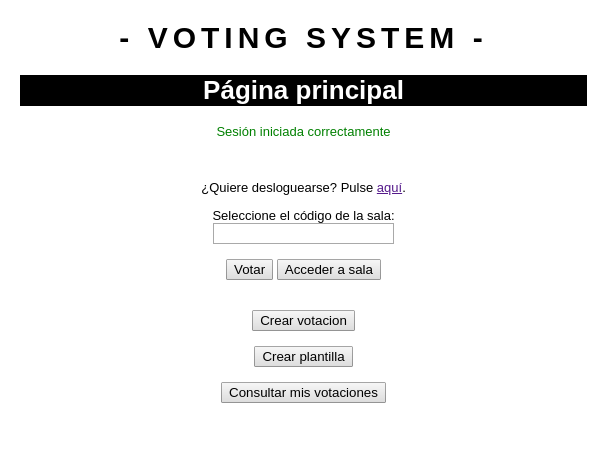
\includegraphics[totalheight=6.6cm]{img/cap8}
 		\caption{}
 	\end{figure}
 
 	Creamos una nueva plantilla para usar en las votaciones:
 	\begin{figure}[H]
 		\centering
 		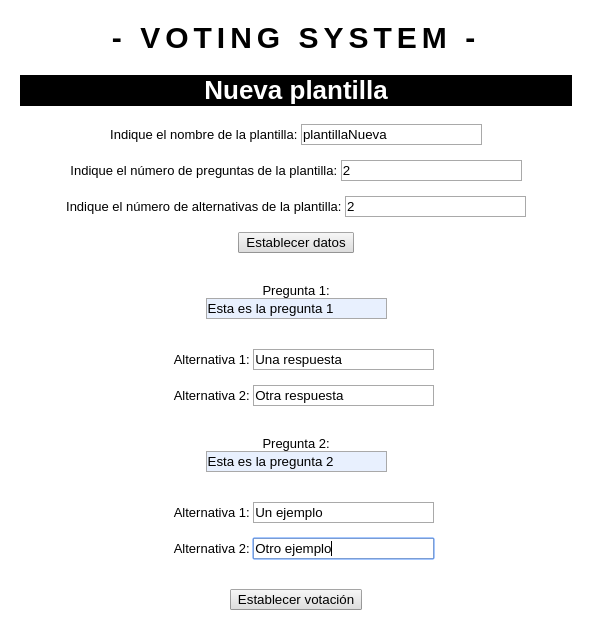
\includegraphics[totalheight=9cm]{img/cap9}
 		\caption{}
 	\end{figure}
 
 	Creamos una nueva votación a partir de la plantilla creada anteriormente:
 	\begin{figure}[H]
 		\centering
 		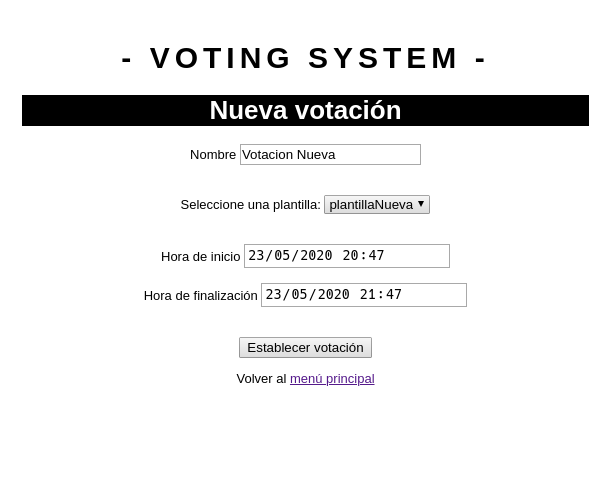
\includegraphics[totalheight=7.5cm]{img/cap10}
 		\caption{}
 	\end{figure}
 
 	Una vez tengamos la votación creada, se genera un mensaje con el código de la sala creada:
 	\begin{figure}[H]
 		\centering
 		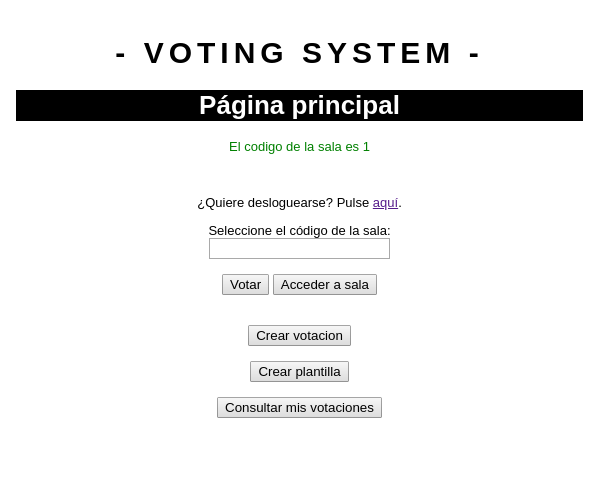
\includegraphics[totalheight=7.5cm]{img/cap11}
 		\caption{}
 	\end{figure}
 
 	Añadimos un usuario nuevo a la votación creada: de esta forma ahora podrán votar tanto \textit{ejemplo} como \textit{ejemplo2}.	
 	\begin{figure}[H]
 		\centering
 		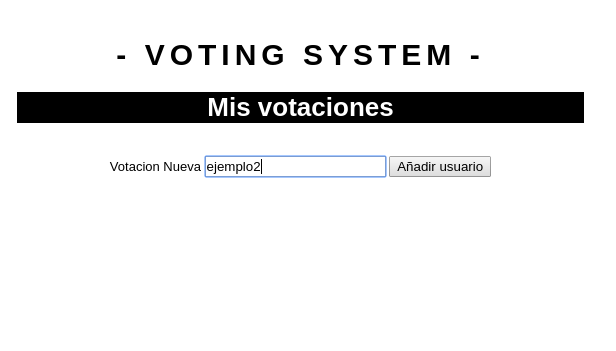
\includegraphics[totalheight=5.6cm]{img/cap19}
 		\caption{}
 	\end{figure}
 
 	\begin{figure}[H]
 		\centering
 		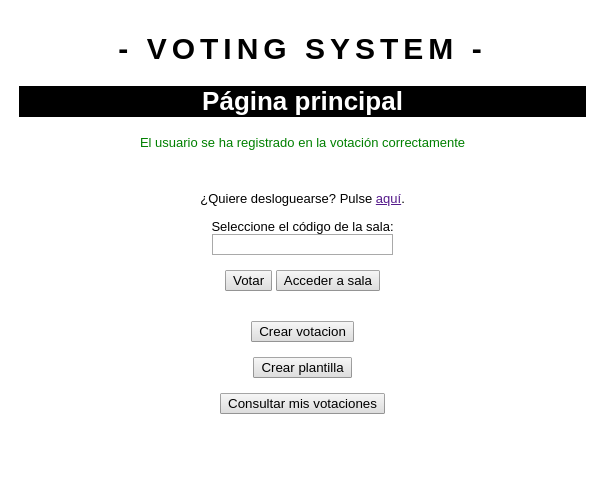
\includegraphics[totalheight=7.6cm]{img/cap12}
 		\caption{}
 	\end{figure}
 	\newpage
 
	 Votamos como usuario \textit{ejemplo}. Es importante que una vez el usuario haya votado, no podrá volver a votar (se notificará el mensaje de error correspondente).
	 Además, también se muestra simultáneamente el resultado de las votaciones en la sala. \\
 
 	\begin{figure}[H]
 		\centering
 		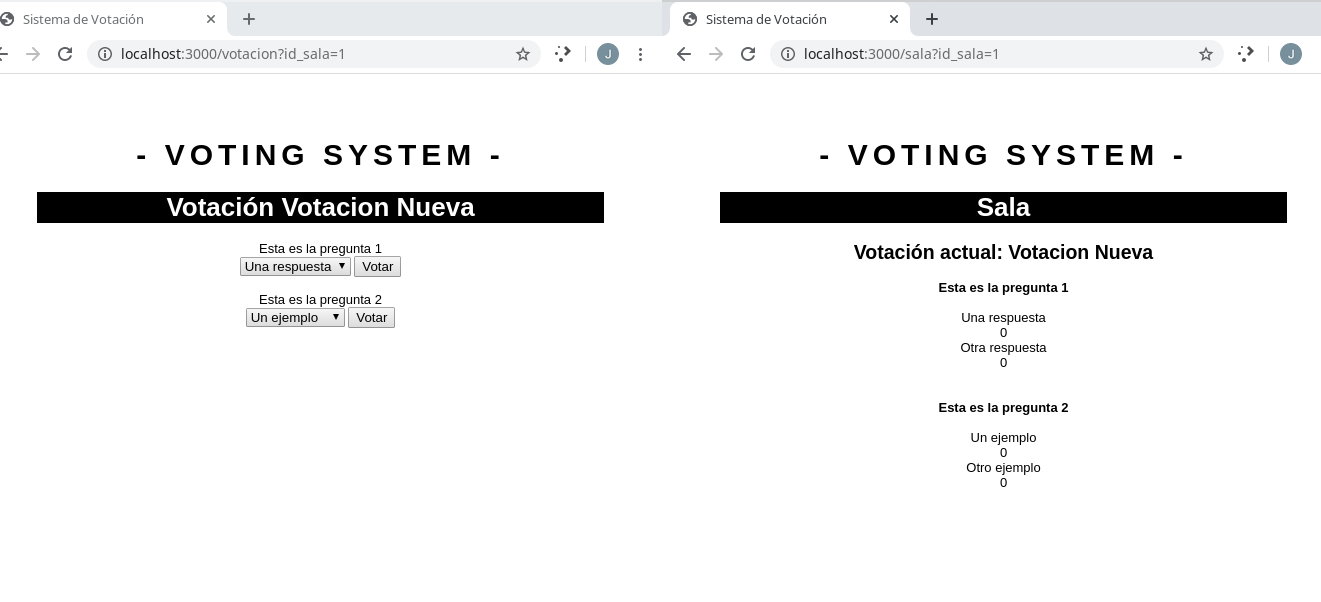
\includegraphics[totalheight=6.5cm]{img/cap13}
 		\caption{}
 	\end{figure}
 
 	\begin{figure}[H]
 		\centering
 		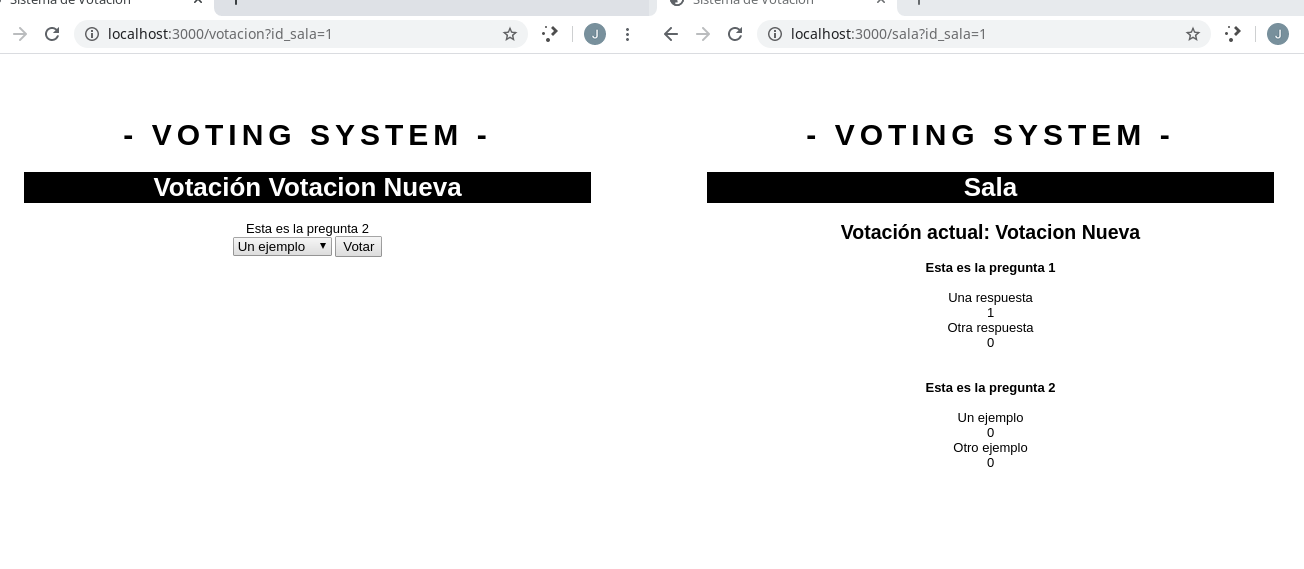
\includegraphics[totalheight=6.5cm]{img/cap14}
 		\caption{}
 	\end{figure}
 
 	\begin{figure}[H]
 		\centering
 		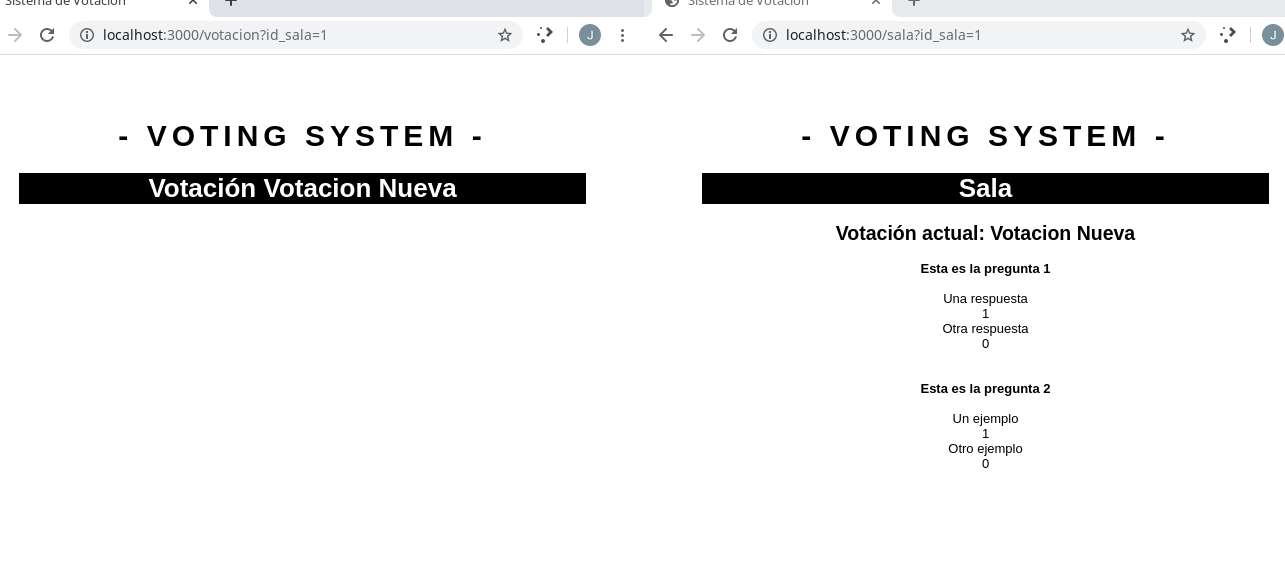
\includegraphics[totalheight=6.34cm]{img/cap15}
 		\caption{}
 	\end{figure}
 
 	A continuación nos deslogueamos, iniciamos sesión como \textit{ejemplo2}, y procedemos a votar: \\
 
 	\begin{figure}[H]
 		\centering
 		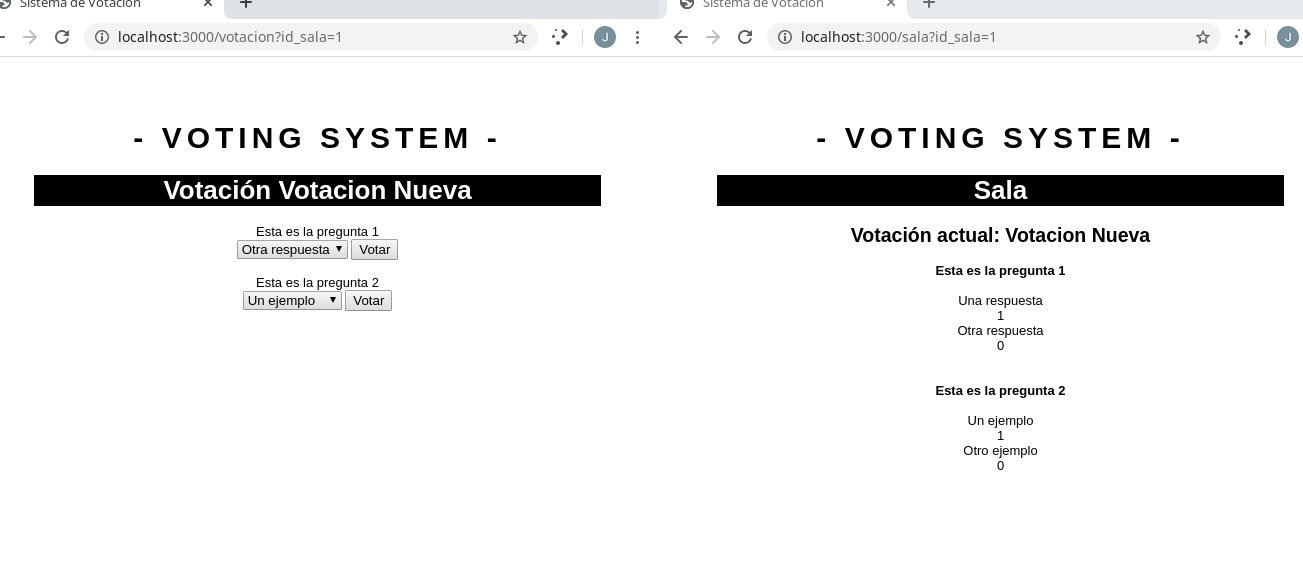
\includegraphics[totalheight=6cm]{img/cap16}
 		\caption{}
 	\end{figure}
 
 
 	\begin{figure}[H]
 		\centering
 		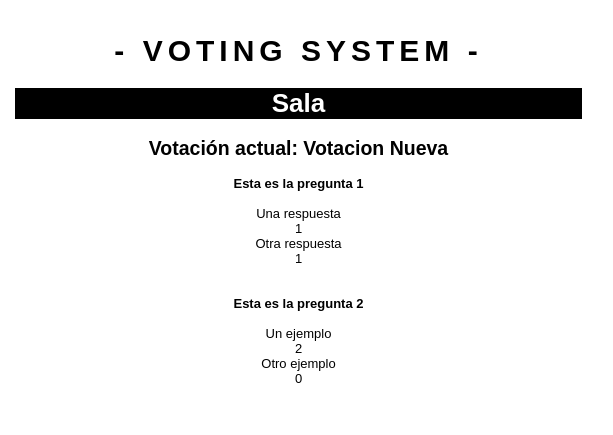
\includegraphics[totalheight=7.2cm]{img/cap17}
 		\caption{}
 	\end{figure}
 
 
	 Finalmente, si iniciamos sesión como otro usuario distinto a \textit{ejemplo1} o \textit{ejemplo2}, se notificará el error correspondiente:
 	\begin{figure}[H]
 		\centering
 		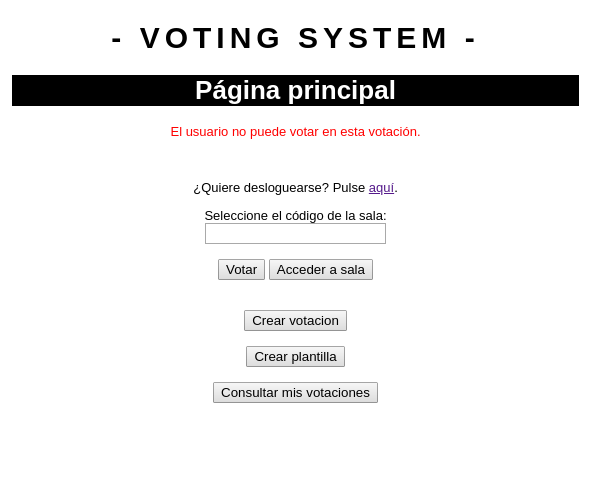
\includegraphics[totalheight=8cm]{img/cap18}
 		\caption{}
 	\end{figure}
 
 	
\end{document}